\chapter{Pairing-Based Contact Discovery}
\label{chap:system}

% TODO redo structure
\paragraph{} In this chapter we present the architecture for our contact discovery scheme (\autoref{sec:architecture}). We then provide outlines of security proofs (\autoref{sec:security}), theoretical performance evaluations (\autoref{sec:performance}) and show how our system maps onto real-world applications such as end-to-end encrypted messaging and mobile-first cryptocurrencies (\autoref{sec:applications}).


\section{Formal problem statement}
\label{sec:probstatement}

\paragraph{} First, we provide a formal definition for the problem of contact discovery. User $A$ is registered to a third-party application from which she receives an opaque account identifier $\acc_A$, an address $\addr_A$ and a secret/public key pair $(\sk_A,\pk_A)$. User $A$ also holds a human-readable discovery identifier $\id_A$ (mobile phone number or an email-address) and a list of contacts. We represent $A$'s address book as a set of discovery identifiers $\contacts{A}$. We assume that users exchanged discovery identifiers through out-of-bound communication but are unable to exchange cryptographic material, including their public keys and addresses. Thus for all users $B$ such that $\id_B \in \contacts{A}$ and $\id_A \in\ \contacts{B}$, $A$ wishes to learn the tuple $(\addr_B, \pk_B)$.

\section{Service architecture}
\label{sec:architecture}

\paragraph{} The foundational design principle for our contact discovery scheme is to provide users with the means to perform contact discovery locally. As we have seen in \autoref{chap:litreview}, sending a client the full list of registered users in a probabilistic data structures such as Bloom and Cuckoo filters requires the client to download and store large amounts of data. Instead, we follow an approach similar to the IBKE protocols and is closely related to the NI-IBKE described in \cite{LRPRF}. Our scheme runs in three phases which we will investigate individually:
\begin{enumerate}
	\item \textbf{Setup:} a one-time step for each user. During the setup phase, a user interacts with the contact discovery service to obtain her unique cryptographic material.
	\item \textbf{Key derivation:} using this cryptographic material, the user is able to compute shared secret keys with any of her contacts knowing only their discovery identifier.	\item \textbf{Discovery:} using their shared secret key, a pair of users can establish a secure meeting point on an untrusted online cache, thus allowing for asynchronous contact discovery.
\end{enumerate}

\noindent \autoref{fig:diagram} shows a diagram of the process described above.

\begin{figure}[H]
	\begin{center}	
	  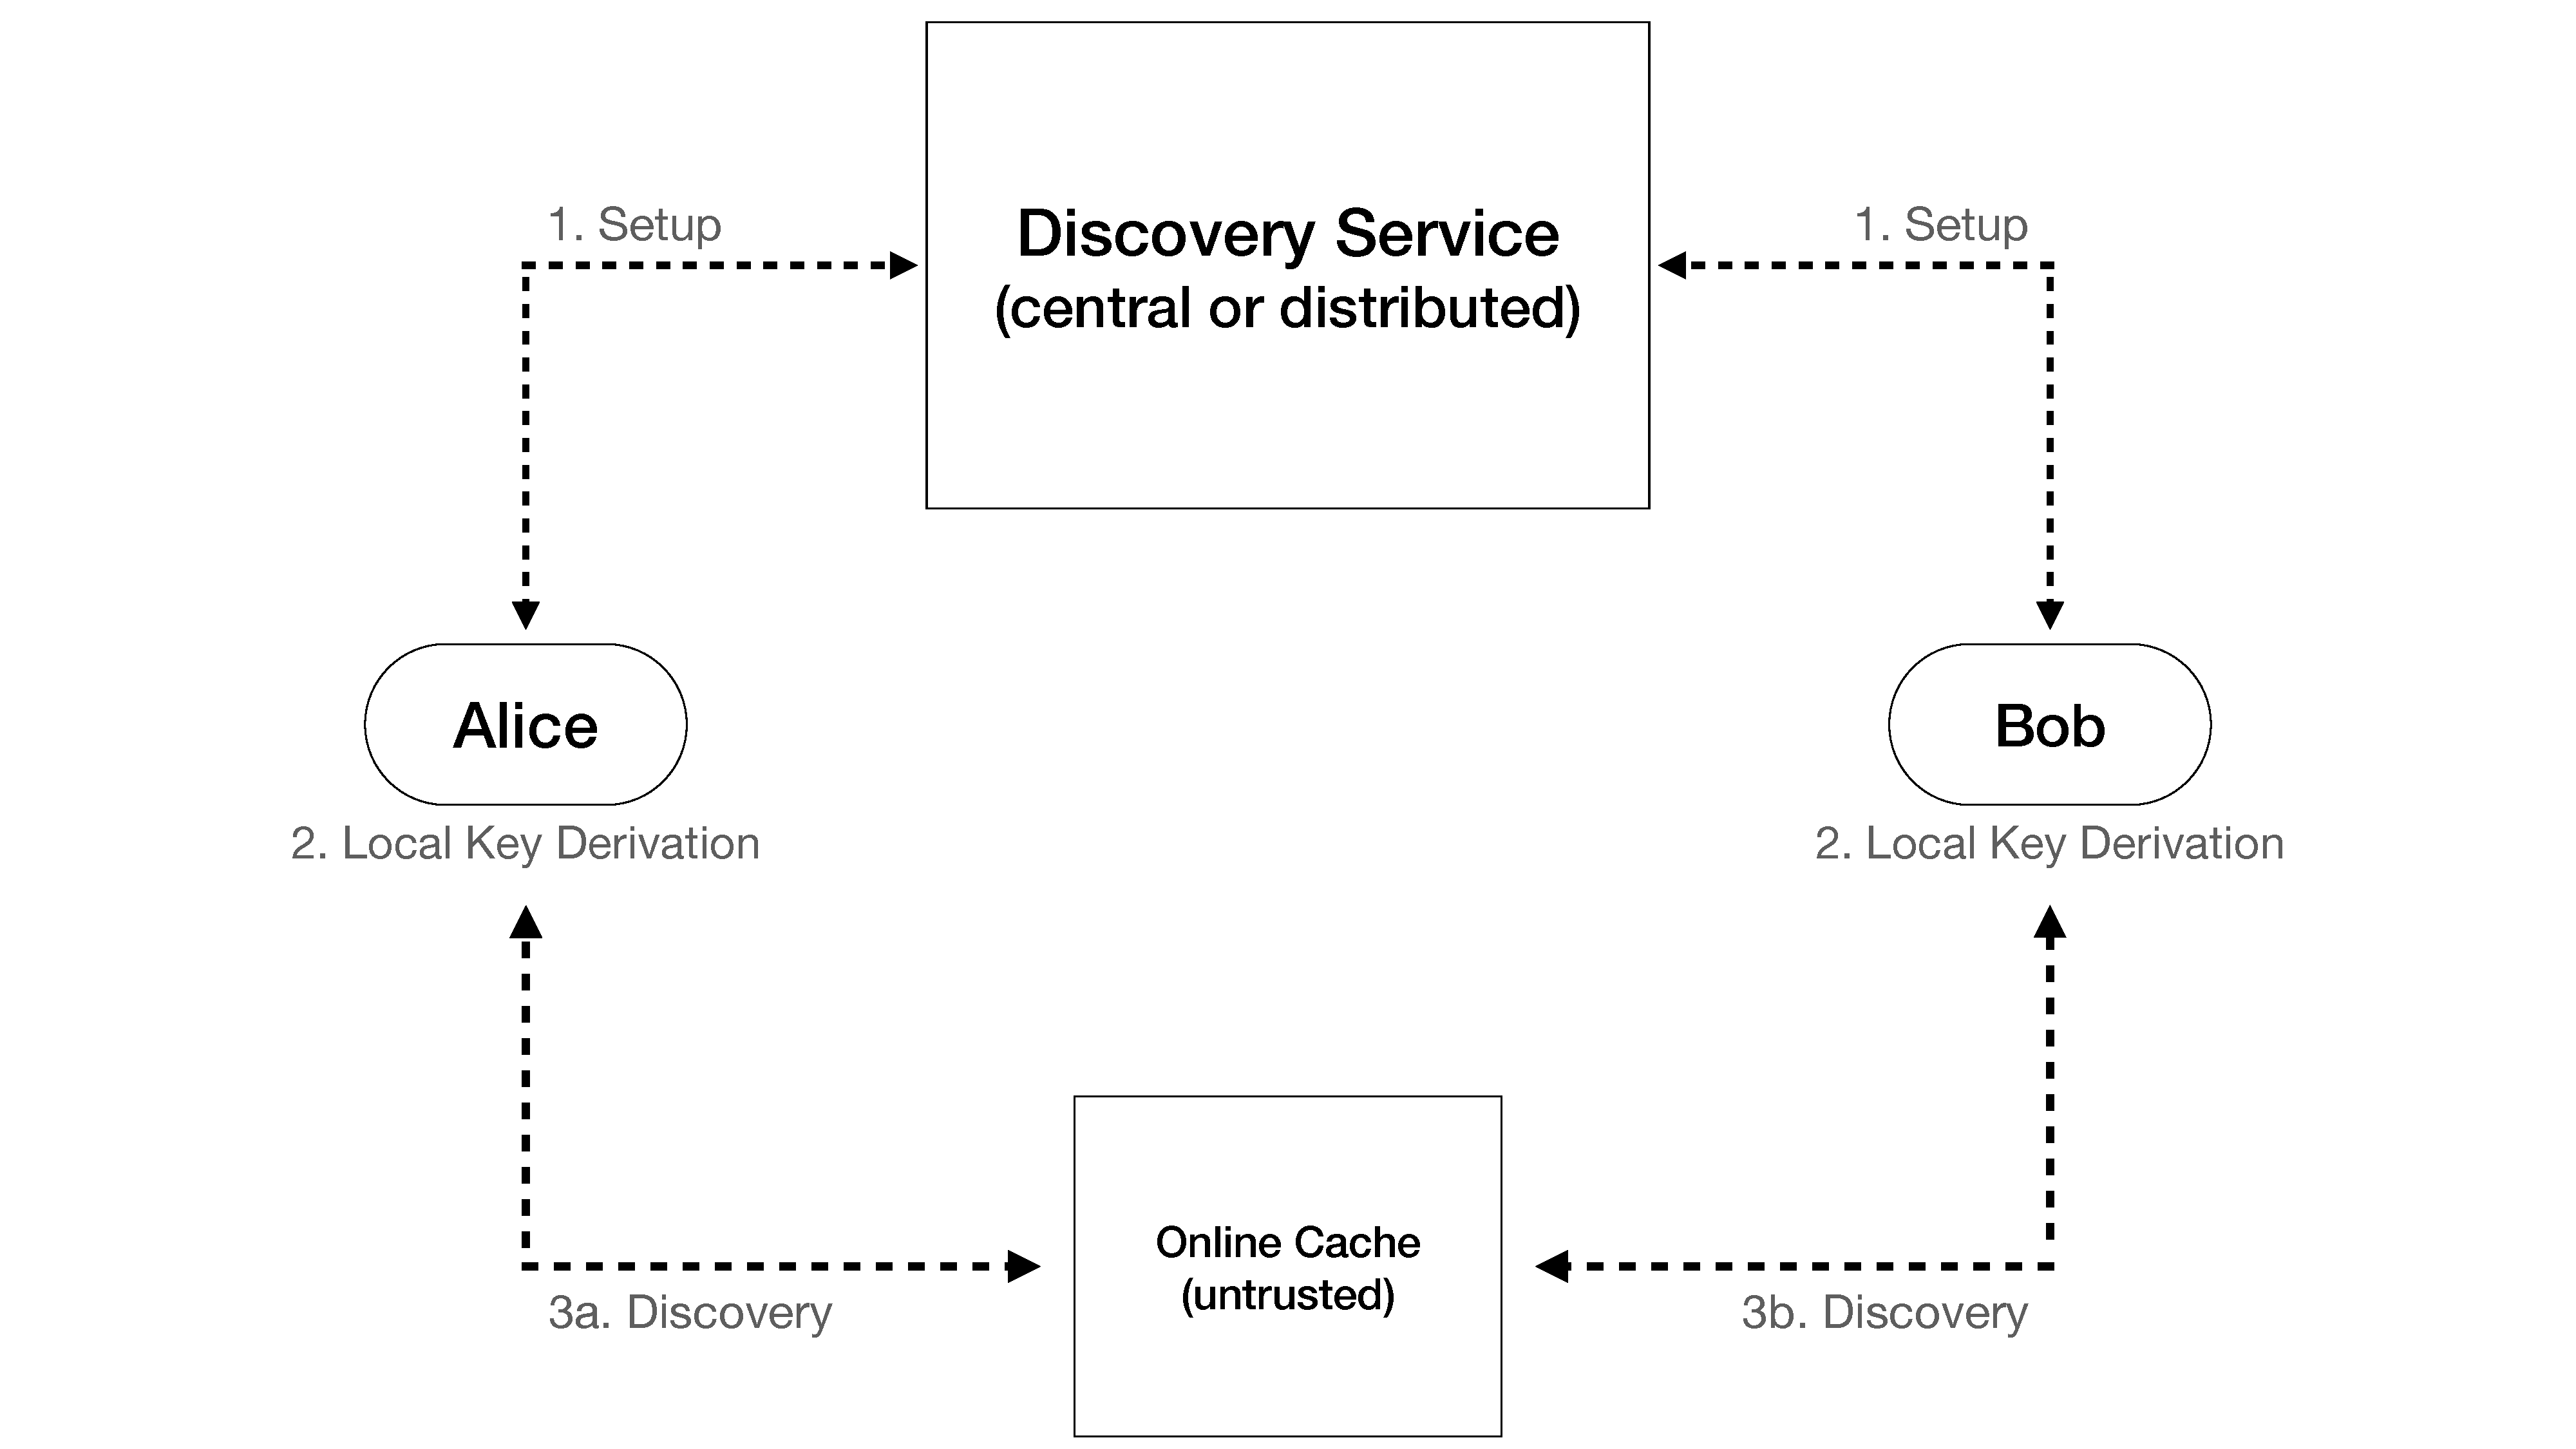
\includegraphics[width=\textwidth]{figures/system}
	  \caption{Contact discovery between a pair of users Alice and Bob, including setup. Numbers indicate the order of execution}
	  \label{fig:diagram}
	 \end{center}
 \end{figure}

	\subsection{Actors, assets and notation}
	
		\noindent We make a brief aside to clarify the actors and assets present in our scheme:		
		\begin{itemize}
			\item \textbf{Users:} each user $A$ holds an opaque account identifier $\acc_A$, an address $\addr_A$, a key pair $(\sk_A,\pk_A)$, a discovery identifier $\id_A$ and an address book $\contacts{A}$ (see \autoref{sec:probstatement}). We denote $\mathcal{ID}$ the set of all existing discovery identifiers.
			\item \textbf{Discovery Service:} the discovery service is a distributed entity. We denote the set of all servers as $\mathcal{S}$ and the $i$-th server as $S_i$. All $n$ servers have jointly executed a $(t,n)$-distributed key generation algorithm such as to hold shares $s_i$ of an unknown master secret key, which we denote $s$. Furthermore, each server holds a list of tuples $(\acc, \pk)$ for all registered users.
			\item \textbf{Online Cache:} the online cache may be operated by the discovery scheme or by a third party and is assumed to be untrusted. Its role is to manage key-value pairs.
			
			\end{itemize}
			
		\noindent Next we define the cryptographic setting for our scheme. For a security parameter $\lambda$:
		\begin{itemize}
			\item $\Gzero, \Gone, \Gt$ are three cyclic groups of prime order $q > 2^{\lambda}$ such that there exists a pairing $e : \Gzero \times \Gone \rightarrow \Gt$.
			\item $H_0: \mathcal{ID}\rightarrow \Gzero$  and $H_1: \mathcal{ID} \rightarrow \Gone$ are two public hash functions modelled as random oracles.
			\item $F: \mathbb{Z}_q \times \mathcal{ID}^2  \rightarrow \Gt$ is a left/right constrained PRF defined as: \begin{equation}
				F(k, (\id_A, \id_B)) = F_k(\id_A, \id_B)= \Pair{H_0(\id_A)}{H_1(\id_B)}^k
			\end{equation}
			\item $\mathbf{KDF}$ is a public, deterministic key derivation function.
			\item $\BTBLS$ is a blind $(t,n)$-threshold BLS signature scheme (see definition \autoref{def:BTBLS}). We denote this scheme's algorithms as $\BTBLS . \Keygen$, $\BTBLS . \Sign$, \textit{etc...} 
			\item $\mathsf{SIG}$ is a strong existentially unforgeable signature scheme which makes use of the third-party provided user keys $(\sk_A,\pk_A)$ and is composed of algorithms $\SIG . \Sign$ and $\SIG . \Verif$.
			\item The master secret key is set to an integer $s \in \mathbb{Z}_q$ chosen uniformly at random. We define two corresponding master public keys ${g_0}^s$ and ${g_1}^s$, for which there exists $i$ public shares denoted as ${g_0}^{s_i}$ and ${g_1}^{s_i}$ respectively.
			\item Let $n$ the number of servers ($n=|\mathcal{S}|$)) and $t$ a fixed threshold such that $1 \leq t \leq n$, we assume that the master secret key is shared according to a secure $t$-out-of-$n$ secret sharing scheme and that no single entity holds the master secret key.
		\end{itemize}

	\subsection{Key derivation}
	
		\paragraph{} We first introduce the essential key derivation step. In doing so, we provide the reader with the necessary material to understand the security constraints under which the initial setup phase operates.
		
		\paragraph{} For all users $B$ such that $\id_B \in \mathcal{C}_A$, user $A$ can compute shared key material with $B$ by evaluating $F_s(\id_A, \id_B)$ and $F_s(\id_B, \id_A)$. From the definition of left/right constrained PRFs, $A$ can do so with the constraining keys $\keyleft{\id_A}$ and $\keyright{\id_A}$:
		\begin{align}
			f_{AB} = F_s(\id_A, \id_B) &= \Pair{\keyleft{\id_A}}{H_1(\id_B)} \\
			f_{BA} = F_s(\id_B, \id_A) &= \Pair{H_0(\id_B)}{\keyright{\id_A}}
		\end{align} 
	
	\noindent Similarly, $B$ can evaluate $F$ at the same points using the constraining keys $\keyleft{\id_B}$ and $\keyright{\id_B}$:		
		\begin{align}
			f_{AB} = F_s(\id_A, \id_B) &= \Pair{H_0(\id_A)}{\keyright{\id_B}} \\
			f_{BA} = F_s(\id_B, \id_A) &= \Pair{\keyleft{\id_B}}{H_1(\id_A)} 
		\end{align}
	
\noindent Using this key material, $A$ and $B$ can establish a symmetric secret key using a standardised key derivation function:
	\begin{equation}
		k_{AB} = k_{BA} = \mathbf{KDF}\left(f_{AB} \xor f_{BA}\right) = \mathbf{KDF}(f_{BA} \xor f_{AB})
	\end{equation}
	
	\paragraph{A note on security --} The constraining keys $\keyleft{\id_A}$ and $\keyright{\id_A}$ allow to compute every symmetric key that $A$ may establish with her contacts. As such, those \textbf{constraining keys must remain private} to $A$. The consequences of a leak range from impersonation to a total leak of $A$'s address book and are further detailed in \autoref{sec:security}.
	
	\subsection{Discovery}
	
		\paragraph{} Using their shared key material $(k_{AB}, f_{AB}, f_{BA})$, users $A$ and $B$ can determine secret memory locations on the online cache to leave an encrypted message for each other. Let $\enc$, $\dec$ be a secure symmetric encryption scheme and $H$ a hash function modelled as a random oracle, we define two cache operations $\mathbf{Write}$ and $\mathbf{Read}$:
		\begin{itemize}
			\item $\mathbf{Write}(f_{AB})$: store the key-value pair $(H(f_{AB}), \enc_{k_{AB}}(\pk_A || \addr_A))$ on the online cache.
			\item $\mathbf{Read}(f_{BA})$: retrieve the key-value pair $(H(f_{BA}), c_{BA})$. If $B$ has already run the discovery phase of our scheme then $c_{BA} = \enc_{k_{BA}}(\pk_B||\addr_B)$. Decrypt $c_{BA}$ using the key $k_{AB} = k_{BA}$.
		\end{itemize}
		
		\paragraph{} Using these two operations, $A$ is able to leave a message for $B$ to find ($\mathbf{Write}$) and check whether $B$ has previously completed the contact matching process ($\mathbf{Read}$ at the address $H(f_{BA})$). Both users regularly check the relevant memory locations for a message. Once both users have completed the contact discovery process, they will hold each other's public keys and address, allowing them to communicate securely.
	
	\subsection{Setup}
	\label{sec:setup}
		
		\paragraph{}  The setup stage serves to provide user $A$ with the constraining keys $k_{\id_A,\mathrm{LEFT}}$ and $k_{\id_A,\mathrm{RIGHT}}$. Consequently, the setup is a security-critical task. As we have shown in \autoref{eq:constrkeys}, under our construction of $F$ the constraining keys can be expressed as:
		\begin{equation}
			k_{\id_A,\mathrm{LEFT}} = H_0(\id_A)^s \quad \mathrm{and} \quad k_{\id_A,\mathrm{RIGHT}} = H_1(\id_A)^s
		\end{equation}
		
		\noindent These constraining keys are equivalent to BLS signatures on $\id_A$ by at least $t$ out of $n$ servers of the discovery service. Notice that the service needs to produce signatures under both variants of the BLS scheme: one with signatures in $\Gzero$ and one with signatures in $\Gone$.
		
		
		\paragraph{} The setup protocol between user $A$ and a server $S_i$ is described as follows:
		\begin{enumerate}
			\item $S_i$ issues a challenge $c$
			\item $A$ chooses a random blinding factor $\alpha \sample \mathbb{Z}_q$ and sends $\acc_A$, $\mathbf{sig}_A \leftarrow \SIG.\Sign(\sk_A, \acc_A || c)$, $\sigma_{\alpha,0} \leftarrow H_0(\id_A)^\alpha$, $\sigma_{\alpha,1} \leftarrow H_1(\id_A)^\alpha$ to $S_i$.
			\item Upon reception of $A$'s request, $S_i$ retrieves the associated public key and checks that the signature $\mathbf{sig_A}$ is valid:
			\begin{equation}
				\SIG.\Verif(\pk_A, \acc_A||c, \mathbf{sig}_A) = 1
			\end{equation}
		\item If the check succeeds, $S_i$ sends $\widehat\sigma_{i,0} \leftarrow {\sigma_{\alpha,0}}^{s_i}$ and $\widehat\sigma_{i,1} \leftarrow {\sigma_{\alpha,1}}^{s_i}$ to $A$.
		\item Using $S_i$'s public keys $({g_0}^{s_i}, {g_1}^{s_i})$, $A$ checks the following equalities:
		\begin{align}
			\Pair{\widehat\sigma_{i,0}}{g_0} &= \Pair{H_0(\id_A)^\alpha}{{g_0}^{s_i}} \\
			\Pair{g_1}{\widehat\sigma_{i,1}} &= \Pair{{g_1}^{s_i}}{H_1(\id_A)^\alpha}
		\end{align}
		\item If the checks succeed (in other words, if $A$ receives valid signatures from the service), $A$ removes the blinding factor $\alpha$ to obtain $H_0(\id_A)^{s_i}$ and $H_1(\id_A)^{s_i}$.
		\end{enumerate}
		
	
	\noindent $A$ repeats the above procedure with at least $t$ servers. Using the obtained signature shares, $A$ can recover the full signatures $H_0(\id_A)^s$ and $H_1(\id_A)^s$ using $\BTBLS.\Combine$.
	
	
	\paragraph{} This completes our description of the contact discovery scheme. We have seen how the setup process allows users to obtain their private constraining keys. Using those keys, users can locally and asynchronously derive shared key material with their contacts by evaluating a left/right constrained PRF at specific points. Finally, using the shared key material, users can leave and read messages from an untrusted online cache, thus completing the contact discovery process.


		
%\fbox{
%	\procedure{Setup}{%
%		\textbf{user } A  \< \<\textbf{server } S \\
%		\alpha \sample \mathbb{Z}_q \< \\
%		\mathbf{sig}_A = \Sign(\sk_A, \acc_A) \< \\
%		\<\sendmessageright{top={$\acc_A,\mathbf{sig}_A, H_0(\id_A)^\alpha, H_1(\id_A)^\alpha$} } \\
%		\<\< \text{If } \Verif(\pk_A, \acc_A, \mathbf{sig}_A) = 0 \\
%		\<\< \qquad\textbf{Abort}\\
%		\<\< \text{Else}\\
%		\< \sendmessageleft{top={$(H_0(\id_A)^\alpha)^s, (H_1(\id_A)^\alpha)^s$}} 
% }
% }


\section{Privacy}
\label{sec:security}


\paragraph{} We will now evaluate the privacy guarantees of our scheme when there are strictly less than $t$ malicious servers. At first, we work under the assumption that discovery identifiers are correctly linked to the users who own them. We then discuss ways in which this assumption can be upheld in practice.





	\subsection{Threat model}
	\paragraph{} An adversary $\Tadv$ wishing to break our scheme's privacy property aims to gain information about the contents of any user's address book. This goal is equivalent to determining whether $\id_B \in \contacts{A}$, for any user $A$ and any identifier $\id_B$ that is not owned by $\Tadv$. $\Tadv$ is characterised as:
	\begin{itemize}
		\item having access to all public information.
		\item having access to the present and past states of the online cache.
		\item may eavesdrop on any communication between the users, servers and online cache.
		\item may spawn any number of users for which $\Tadv$ owns the discovery identifier.
		\item may control up to $t-1$ servers in the discovery service.
	\end{itemize}
	
	\subsection{Proof outline}
	
	\paragraph{} To guide our analysis, we provide an attack tree\footnote{as defined by Schneier \cite{attacktree}} against the privacy property of our scheme in \autoref{fig:attacktree}. The root node represents the attacker's goal and each child node represents an option to solve the problem indicated in the parent node. Consequently leaf nodes represent the attacker's entry points: breaking the security of $F$, obtaining the master secret key $s$, forging BLS signatures on another user's discovery identifier, impersonating a user or computing the shared key material $(k_{AB}, f_{AB}, f_{BA})$. We will therefore consider each leaf node and show that our scheme is resistant against these attacks.
	
	
		\begin{figure}[H]
			\begin{center}
				\begin{center}
	

\begin{forest}
for tree={
  draw,
  minimum height=1cm,
  anchor=north,
  align=center,
  child anchor=north
},
[{Learn whether $\id_B \in \contacts{A}$}, align=center, name=SS
  [{Distinguish key-value pair\\ $(H(f_{AB}), \enc_{k_{AB}}(\pk_A || \addr_A))$\\ on online cache from random}, name=PDC
    [{Distinguish $f_{AB}$ from random}
    	[Break security\\ property of $F$\\ (definition \autoref{def:lrPRFsec})]
    	[Obtain $s$]
    	[{Obtain $A$'s\\ constraining keys}
    		[Forge BLS signatures]
    		[Impersonate $A$]
    	]
    ]
    [Decrypt $\enc_{k_{AB}}(\pk_A || \addr_A))$
    	[Compute $k_{AB}$]
    ]
  ]
]
\end{forest}

\end{center}
				\caption{Attack tree against our discovery scheme. Branches represent ``OR'' statements}
				\label{fig:attacktree}
			\end{center}
		\end{figure}

	
	
%		\paragraph{} Our scheme reduces the contact discovery problem to the evaluation of a left/right constrained PRF at two specific points, namely $(\id_A, \id_B)$ and $(\id_B, \id_A)$. Indeed an adversary trying to uncover a link between users $A$ and $B$ without computing their shared key material will face two obvious hurdles. Firstly, such an adversary will be unable to find $A$ and $B$'s meeting point on the online cache other than by exhaustively iterating through all possible location. Furthermore, since $H$ is modelled as a random oracle, this adversary will be unable to distinguish this location from any other. The second issue is that the value stored in that location is encrypted under $k_{AB}$. Therefore, to uncover the link between $A$ and $B$, an adversary will need to evaluate the left/right constrained PRF at the correct points.
		
		
%		\paragraph{} We provide a formal definition of secure left/right constrained PRFs by using an attack game. We will then show that the construction used in our scheme meets the security definition.
		
		\subsubsection{Security of our PRF construction}
		
		\paragraph{} We will first show that our construction for the left/right constrained PRF using an asymmetric pairing is secure as per definition \autoref{def:lrPRFsec}. Our construction is closely related to the one presented by Boneh and Waters \cite{LRPRF}. As such our proof sketch makes use of very similar ideas.
		
		\begin{theorem}
			The PRF $F$ defined as $F(k, (x,y)) = \Pair{H_0(x)}{H_1(y)}^k$ is a secure constrained PRF with respect to its constraining keys assuming the decisional bilinear Diffie-Hellman assumption holds for $e$ and the functions $H_0$ and $H_1$ are modelled as random oracles.
		\end{theorem}
		
		\begin{proof}[\textbf{Proof sketch}]
			We assume for contradiction the existence of a probabilistic polynomial-time adversary $\adv$ that distinguishes $F$ from random as in definition \autoref{def:lrPRFsec}, however $\adv$ is limited to a single $\mathsf{Challenge}$ query. We can then construct an adversary $\bdv$ that breaks the decisional bilinear Diffie-Hellman (DBDH) assumption.\\
			
			Given $(g_0, g_1, u_0 \leftarrow {g_0}^\alpha, u_1 \leftarrow {g_1}^\alpha, v_0 \leftarrow {g_0}^\beta, w_1 \leftarrow {g_1}^\gamma, z^{(b)})$, $\bdv$'s goal is to determine whether $z^{(b)} = z^{(0)} = {g_0}^{\alpha\beta\gamma}$ or $z
			^{(b)} = z^{(1)} = {g_0}^\delta$, where $\delta \sample \mathbb{Z}_q$ (see Attack Game \autoref{att:DBDH} in \autoref{ap:coCDH}). Using the pairing operation, this game can be viewed as distinguishing the output of $F$ from a random element of $\Gt$. Indeed let $b,c \in \mathcal{X}$ such that $H_0(b) = {g_0}^\beta$ and $H_1(c) = {g_1}^\gamma$, then:
			\begin{equation}
				\Pair{\Smallz{b}}{g_1} =
				\begin{cases} \Pair{g_0}{g_1}^{\alpha\beta\gamma} = \Pair{{g_0}^\beta}{{g_1}^\gamma}^\alpha =  F(\alpha, (b, c)), & \text{if } b=0 \\
				 \Pair{g_0}{g_1}^\delta	= {g_T}^\delta, & \text{if } b=1
				\end{cases}
			\end{equation}
			Thus, $\bdv$ will run $\adv$ as a sub-routine and must therefore emulate its oracles, namely $F.\mathsf{eval}$, $F.\mathsf{constrain}$, $\mathsf{Challenge}$ and oracles for the hash functions $H_0,H_1$. \\
			
			When $\adv$ issues a query to $H_0(x)$, $\bdv$ chooses a consistent random $\widehat x \sample \mathbb{Z}_q$ and sets $H_0(x) \leftarrow {g_0}^{\widehat x}$. To one of $\adv$'s queries to $H_0$ which we denote $x^*$, $\bdv$ responds with $H_0(x^*) \leftarrow v_0$. Queries to $H_1$ are answered in a similar fashion where one query is responded to with $H_1(y^*) \leftarrow w_1$. Using these values, queries to $F.\mathsf{constrain}(x,LEFT)$ where $x\neq x^*$ are answered with $k_{x,LEFT} \leftarrow  {u_0}^{\widehat x}$. Notice that as required
				$$ {u_0}^{\widehat x} = ({g_0}^\alpha)^{\widehat x} = {g_0}^{\alpha \widehat x} = ({g_0}^{\widehat x})^{\alpha} = H_0(x)^\alpha$$
			Similarly, queries to $F.\mathsf{constrain}(y,RIGHT)$ where $y\neq y^*$ are answered with $k_{y,RIGHT} \leftarrow  {u_1}^{\widehat y}$. Queries to $F.\mathsf{eval}(x,y)$ are answered for $x \neq x^*$ or $y \neq y^*$ by building the constraining keys as it is done for the $F.\mathsf{constrain}$ oracle. Notice that $\bdv$ does not hold the values $\beta,\gamma$ and is therefore unable to answer queries to the $F.\mathsf{constrain}$ oracle for $(x^*, LEFT)$ and $(y^*, RIGHT)$, nor can it answer the $F.\mathsf{eval}$ query for $(x^*,y^*)$. This is in fact equivalent to starting Attack Game \autoref{att:lrPRF} with the set $C$ initialised to $\{(x^*,y^*)\}$. \\
			
			After $n$ queries to the $H_0$ oracle and $m$ queries to the $H_1$ oracle, $\adv$ will hold at most $n \times m$ pairs on which it could challenge.	 Some of these pairs may have been added to the set $V$ due to queries to $F.\mathsf{constrain}$ and $F.\mathsf{eval}$, and thus become ineligible for challenging. However, since the experiment started with $C = \{(x^*,y^*)\}$, we can be sure that $(x^*,y^*)$ is an eligible pair (remember that the attack game maintains the invariant $C \cap V = \emptyset$). Therefore, $\adv$ will challenge the pair $(x^*,y^*)$ with probability $p \geq \frac{1}{n\times m}$, to which $\bdv$ answers with $\Smallz{b}$. 
			
			If $b=0$, then $\Smallz{b} = F(\gamma, (x^*, y^*))$ and $\adv$ will answer as in experiment EXP(0). On the other hand if $b=1$, then $\Smallz{b} = {g_T}^{\delta}$ and $\adv$ will answer as in experiment EXP(1). Let $b'_\adv$ be the output of $\adv$, we define as $b'_\bdv \leftarrow b'_\adv$ the return value of $\bdv$. Thus
			\begin{equation}
				\Pr[b'_\bdv = b] \geq \frac{1}{n \times m} \times \Pr[b'_\adv = b]
			\end{equation}
			
			Given that $\adv$ is a probabilistic polynomial-time adversary, $n \times m$ must necessarily be polynomial in $\lambda$. Therefore, if $\adv$'s advantage is non-negligible then so is $\bdv$'s, thus breaking the DBDH assumption and yielding a contradiction.
		\end{proof}
		
\subsubsection{Computing $A$ and $B$'s shared key material}

\paragraph{} To compute $A$ and $B$'s shared key material, an attacker needs to compute $f_{AB}$ and $f_{BA}$. This is in fact a harder problem than the decisional problem investigated above. We have already shown that no probabilistic polynomial-time adversary can break the security of $F$ under the DBDH assumption. Similarly, no probabilistic polynomial-time adversary will be able to compute either $f_{AB}$ or $f_{BA}$ under the DBDH assumption without access to the relevant constraining keys or the master secret key.

\subsubsection{Obtaining the master secret key}

\paragraph{} Next, we consider the option for an attacker to obtain the master secret key $s$. It is part of our assumption that there are strictly less than $t$ malicious servers. Therefore, they do not meet the threshold required to construct the master secret key. An attacker aiming to break our scheme through this attack will need to steal at least one of the key shares.

\subsubsection{Forging a BLS signature}

\paragraph{} As we have seen in \autoref{sec:setup}, the service generates constraining keys by signing a user's discovery identifier. The signing algorithm is a blind $(t,n)$-threshold BLS algorithm. As per \autoref{th:blsforge}, the BLS signature is existentially unforgeable against chosen message attacks under the co-Computational Diffie Hellman assumption. This assumption is in fact a weaker than the DBDH assumption which is required for the left/right constrained PRF security.


\subsubsection{Impersonating a user}

\paragraph{} Impersonation attacks are the most threatening to our scheme and lead to open questions. We first describe the issue and offer two solutions, neither of which are fully satisfying. The attack is performed by running the setup process maliciously from the user side: upon receiving a challenge $c$, $\Tadv$ can send the tuple $(\acc_{\Tadv}$, $\SIG.\Sign(\sk_{\Tadv}, \acc_{\Tadv}||c)$, $H_0(\id_A)^\alpha$, $H_1(\id_A)^\alpha$). The server $S_i$ receiving this tuple will find that the signature $\SIG.\Sign(\sk_{\Tadv}, \acc_{\Tadv}||c)$ does verify for the specified account and challenge. Furthermore, $S_i$ will be unable to distinguish the blinded values $H_0(\id_A)^\alpha, H_1(\id_A)^\alpha$ from random elements in $\Gzero$ and $\Gone$ respectively. As such $S_i$ will issue partial constraining keys for $\id_A$ to $\Tadv$. Repeating this process with $t$ servers, $\Tadv$ will obtain the full constraining keys for user $A$.

\paragraph{} The first solution is for $A$ to transmit her discovery identifier in clear to $S_i$. The server can then use out-of-bound communication to verify that $A$ indeed owns $\id_A$ (possible techniques include sending a one-time code via text message or email). If $A$ proves that she owns $\id_A$, $S_i$ provides the partial signatures for that discovery identifier. Notice that under this approach, $A$ cannot blind the hash of her discovery identifier. Consequently, the communication between $A$ and $S_i$ must be encrypted to prevent an eavesdropping adversary from learning the signature share on $\id_A$. Furthermore, this identification method allows the servers to build a list of identifiers for the users registered to the mobile application. In some cases, this may be a breach of privacy.

\paragraph{} The second solution makes use of identification tokens to delegate the task of linking a user to their discovery identifier. Suppose an entity $V$ (centralised or distributed) is trusted to verify whether a user owns a discovery identifier. Using a secret key $v \sample \mathbb{Z}_q$ and the corresponding public keys ${g_0}^v$ and ${g_1}^v $, $V$ could issue ownership tokens in the form of BLS signatures $t_{0,A}= H_0(\id_A)^v, t_{1,A}=H_1(\id_A)^v$. These tokens can then be blinded and verified against a blinded discovery identifier $H_0(\id_A)^\alpha, H_1(\id_A)^\alpha$:
\begin{align}
\label{eq:token0}
	\Pair{{t_{0,A}}^\alpha}{g_1} = \Pair{H_0(\id_A)^\alpha}{{g_1}^v} &\iff t_{0,A} = H_0(\id_A)^v \\
	\label{eq:token1}
	\Pair{g_0}{{t_{1,A}}^\alpha} = \Pair{{g_0}^v}{H_1(\id_A)^\alpha} &\iff t_{1,A} = H_1(\id_A)^v
\end{align}

\noindent Users can therefore send ${t_{0,A}}^\alpha$, ${t_{1,A}}^\alpha$ along with the setup tuple $(\acc_A$, $\mathbf{sig}_A$, $H_0(\id_A)^\alpha$, $H_1(\id_A)^\alpha)$, to allow each server to perform the checks in \autoref{eq:token0} and \autoref{eq:token1}. 

\paragraph{} While this method allows identification without revealing the discovery identifier to the contact discovery servers, it relies on a trusted verification entity $V$. In fact, this entity faces the same problem we were trying to avoid: it must output a BLS signature on an identifier only if the request was made by the identifier's owner. This raises the question of trust within our system. The contact discovery scheme can be made secure and oblivious to which user owns which discovery identifier. However, for that to happen, we need another entity to perform that check and gather private information about the users.

	\subsection{Consequences of a breach}
	


\section{Theoretical performance evaluation}
\label{sec:performance}


\section{Applications}
\label{sec:applications}

	\subsection{End-to-end encrypted messaging}
	
	\subsection{Mobile-first cryptocurrencies}
